\documentclass[11pt,a4paper]{article}
\usepackage[T1]{fontenc}
\usepackage[utf8]{inputenc}
\usepackage[margin=23mm]{geometry}
\usepackage{amsmath,amssymb,booktabs,longtable,array,xurl,graphicx,hyperref}
\usepackage{tikz}
\usetikzlibrary{arrows.meta,patterns}
% Generated from results/elm/elm_example.h5; do not edit values.
\newcommand{\elmAcceptance}{0.10961179}
\newcommand{\elmBlueForwardPerThousand}{35.62383316}
\newcommand{\elmBlueSiPMPerThousand}{11.87461105}
\newcommand{\elmBlueTotalPerThousand}{71.24766633}
\newcommand{\elmBucketNS}{250.00000000}
\newcommand{\elmCapture}{0.33333333}
\newcommand{\elmChannelDiameterMM}{3.50000000}
\newcommand{\elmClipThresholdPE}{4334.38130171}
\newcommand{\elmCurrentLimitMA}{1.00000000}
\newcommand{\elmDarkOnlyMicrocells}{18176.00000000}
\newcommand{\elmDarkRateKCPS}{700.00000000}
\newcommand{\elmDriftEndKV}{31.20000000}
\newcommand{\elmELDropKV}{15.00000000}
\newcommand{\elmELFieldKVcm}{30.00000000}
\newcommand{\elmEntryKV}{31.50000000}
\newcommand{\elmExitKV}{46.50000000}
\newcommand{\elmFieldRatio}{100.00000000}
\newcommand{\elmForwardFactor}{0.50000000}
\newcommand{\elmGain}{360000.00000000}
\newcommand{\elmGradingKVcm}{4.65000000}
\newcommand{\elmHeExitPhotons}{137.12435474}
\newcommand{\elmHePrimaryPE}{4.75364430}
\newcommand{\elmHeSiPMPhotons}{14.85513843}
\newcommand{\elmHeYield}{1251.00000000}
\newcommand{\elmHexAperturePercent}{35.42576883}
\newcommand{\elmIlluminatedMicrocells}{21808.00000000}
\newcommand{\elmMicrocells}{39984.00000000}
\newcommand{\elmNoisePE}{3.54166667}
\newcommand{\elmOpticalFraction}{0.01187461}
\newcommand{\elmOpticalPercent}{1.18746111}
\newcommand{\elmOptimumGlueIndex}{1.53460093}
\newcommand{\elmPDE}{0.32000000}
\newcommand{\elmRecoveryNS}{12.50000000}
\newcommand{\elmReducedGrading}{0.31000000}
\newcommand{\elmSquareAperturePercent}{30.67961576}
\newcommand{\elmThreeELDrop}{22.50000000}
\newcommand{\elmThreeExit}{54.00000000}
\newcommand{\elmThreeLength}{11.61290323}
\newcommand{\elmTrappingAngleDeg}{48.18968510}
\newcommand{\elmTwoELDrop}{15.00000000}
\newcommand{\elmTwoExit}{46.50000000}
\newcommand{\elmTwoHalfELDrop}{18.75000000}
\newcommand{\elmTwoHalfExit}{50.25000000}
\newcommand{\elmTwoHalfLength}{10.80645161}
\newcommand{\elmTwoLength}{10.00000000}
\newcommand{\elmVUVExitPerThousand}{109.61179435}
\newcommand{\elmWebMM}{0.50000000}
\newcommand{\elmXeExitPhotons}{143.03516272}
\newcommand{\elmXePrimaryPE}{4.95855231}
\newcommand{\elmXeSiPMPhotons}{15.49547596}
\newcommand{\elmXeYield}{1304.92492676}
\newcommand{\elmPilotFourEvents}{100.00000000}
\newcommand{\elmPilotFourRetained}{97.00000000}
\newcommand{\elmPilotFourASICLoss}{0.01653848}
\newcommand{\elmPilotFourFullRMS}{0.33601370}
\newcommand{\elmPilotFourRetainedRMS}{0.29278993}
\newcommand{\elmPilotFourUnclippedRMS}{0.29418002}
\newcommand{\elmPilotFourMeanPE}{76.23343945}
\newcommand{\elmPilotFourMaxPE}{1249.83000000}
\newcommand{\elmPilotFiveEvents}{100.00000000}
\newcommand{\elmPilotFiveRetained}{89.00000000}
\newcommand{\elmPilotFiveASICLoss}{0.21840377}
\newcommand{\elmPilotFiveFullRMS}{0.93964321}
\newcommand{\elmPilotFiveRetainedRMS}{0.22580260}
\newcommand{\elmPilotFiveUnclippedRMS}{0.23465510}
\newcommand{\elmPilotFiveMeanPE}{121.65243003}
\newcommand{\elmPilotFiveMaxPE}{1994.41000000}

\newcommand{\num}[2][3]{\pgfmathprintnumber[fixed,precision=#1,fixed zerofill]{#2}}
\hypersetup{colorlinks=true,linkcolor=blue,urlcolor=blue,citecolor=blue}
\newcommand{\code}[1]{\path{#1}}
\newcommand{\EP}{\mathcal{E}_{\mathrm{EL}}}
\newcommand{\gradV}{G_{\mathrm{M}}}
\title{ELM: electroluminescence and light-guide manifold}
\author{NAUSICAA design note}
\date{5 November 2026}
\begin{document}
\maketitle

\section{Purpose and configuration}
The EL manifold (ELM) combines an electroluminescence section with a downstream
optical and voltage-grading section. Electrons from the TPC enter holes in an
acrylic structure with copper-coated electrode faces. Electroluminescence (EL)
is produced inside those holes. Each hole faces a light-guide rod whose entrance
is coated with tetraphenyl butadiene (TPB). Converted visible light is transported
to a SiPM at the grounded end of the rod. Each rod is surrounded by a continuous
xenon-filled annulus. Acrylic fills the space between those gas channels and
is treated as opaque to incident VUV light in this design. The gas annulus
provides the low-index boundary for total internal reflection (TIR).

The geometry and operating values below are user design inputs. They define a
adopted configuration for production and parameter scans. Hole diameter, hole
pitch, EL thickness, rod length, SiPM dimensions, pressure, fields, optical
properties and sensor response are configurable. One guide and one sensor per
EL hole define the initial channel arrangement.

The adopted baseline has 2.5 mm diameter holes and rods on a 4 mm pitch,
a 0.5 mm radial xenon gap around each rod, and centred $3\times3$ mm$^2$
Hamamatsu S14160-3015PS SiPMs. The TPB conversion efficiency is 0.65. Norland NOA 87 couples the
polished rod exit to the SiPM window. Electron collection is set to unity
for $\EP\geq2$ kV/cm/bar in this geometry. The optical baseline uses isotropic
emission inside the guide, meridional trapping, lossless propagation and
unit coupling transmission. These are the agreed calculation assumptions.
Figure~\ref{fig:elm} defines the geometry.

\begin{figure}[p]
\centering
\resizebox{\linewidth}{!}{% Editable vector drawing. Longitudinal scale is schematic.
% Rod diameter and radial gas gap share a transverse scale: 2 units = 2.5 mm.
% Thus each 0.5 mm annulus is 0.4 unit in the longitudinal panel.
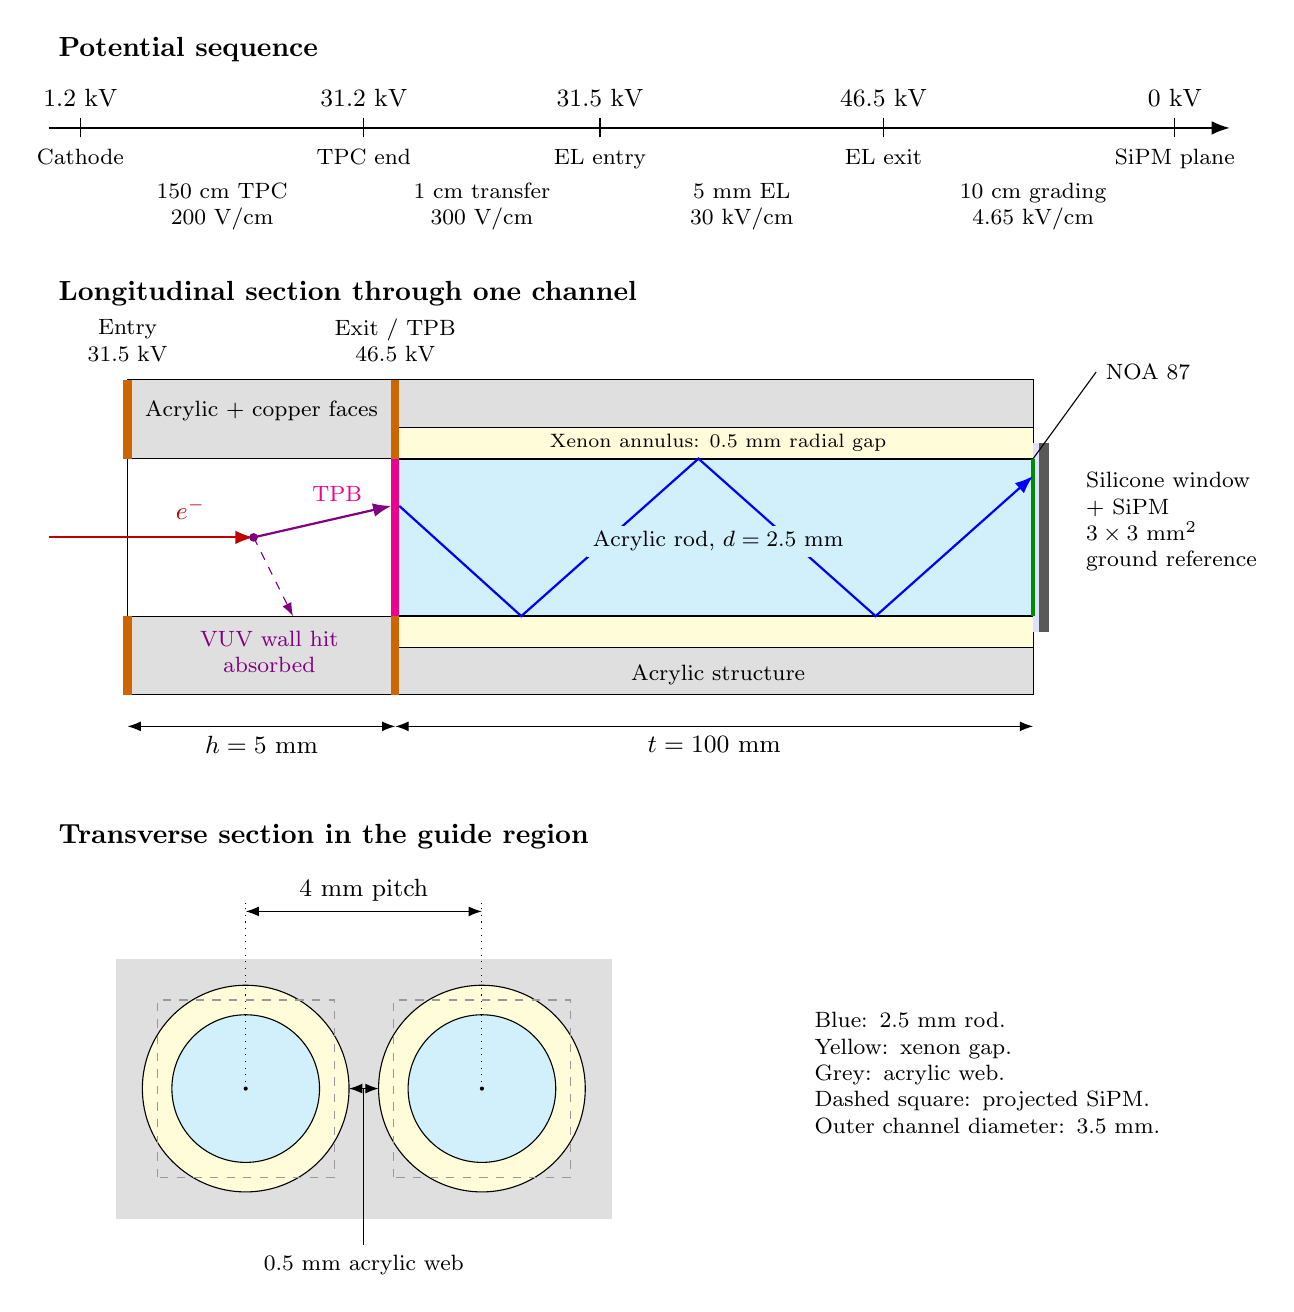
\begin{tikzpicture}[x=1cm,y=1cm,font=\small,>=Latex]
\node[anchor=west,font=\bfseries] at (0,1.0) {Potential sequence};
\draw[->,thick] (0,0)--(15,0);
\foreach \x/\v/\lab in {0.4/1.2/Cathode,4/31.2/TPC end,7/31.5/EL entry,10.6/46.5/EL exit,14.3/0/SiPM plane}{
  \draw (\x,-.12)--(\x,.12);
  \node[above,align=center] at (\x,.15) {\v\ kV};
  \node[below,align=center,font=\footnotesize] at (\x,-.15) {\lab};
}
\node[font=\footnotesize,align=center] at (2.2,-1.0) {150 cm TPC\\200 V/cm};
\node[font=\footnotesize,align=center] at (5.5,-1.0) {1 cm transfer\\300 V/cm};
\node[font=\footnotesize,align=center] at (8.8,-1.0) {5 mm EL\\30 kV/cm};
\node[font=\footnotesize,align=center] at (12.5,-1.0) {10 cm grading\\4.65 kV/cm};

\node[anchor=west,font=\bfseries] at (0,-2.1) {Longitudinal section through one channel};
% Hole block and acrylic manifold, with a gas-filled channel around the rod.
\fill[gray!25] (1,-3.2) rectangle (4.4,-7.2);
\fill[white] (1,-4.2) rectangle (4.4,-6.2);
\draw (1,-3.2) rectangle (4.4,-7.2);
\draw (1,-4.2)--(4.4,-4.2) (1,-6.2)--(4.4,-6.2);
\fill[gray!25] (4.4,-3.2) rectangle (12.5,-7.2);
\fill[yellow!15] (4.4,-3.8) rectangle (12.5,-6.6);
\fill[cyan!18] (4.4,-4.2) rectangle (12.5,-6.2);
\draw (4.4,-3.2) rectangle (12.5,-7.2);
\draw (4.4,-3.8)--(12.5,-3.8) (4.4,-6.6)--(12.5,-6.6);
\draw[thick] (4.4,-4.2)--(12.5,-4.2) (4.4,-6.2)--(12.5,-6.2);
% Copper-coated EL faces, opening onto the gas hole.
\draw[orange!80!black,line width=3pt] (1,-3.2)--(1,-4.2) (1,-6.2)--(1,-7.2);
\draw[orange!80!black,line width=3pt] (4.4,-3.2)--(4.4,-4.2) (4.4,-6.2)--(4.4,-7.2);
\draw[magenta,line width=3pt] (4.4,-4.2)--(4.4,-6.2);
% Glue / packaged sensor front window / active sensor.
\fill[blue!12] (12.5,-4.0) rectangle (12.58,-6.4);
\fill[black!65] (12.58,-4.0) rectangle (12.70,-6.4);
\draw[green!55!black,line width=1.5pt] (12.5,-4.2)--(12.5,-6.2);
\draw[red!75!black,->,thick] (0,-5.2)--(2.6,-5.2);
\node[red!75!black,above] at (1.8,-5.1) {$e^-$};
\fill[violet] (2.6,-5.2) circle (.055);
\draw[violet,->,thick] (2.6,-5.2)--(4.35,-4.8);
\draw[violet,->,dashed] (2.6,-5.2)--(3.1,-6.2);
\node[violet,font=\footnotesize,align=center] at (2.8,-6.65) {VUV wall hit\\absorbed};
\draw[blue,->,thick] (4.45,-4.8)--(6.0,-6.2)--(8.25,-4.2)--(10.5,-6.2)--(12.5,-4.42);
\node[font=\footnotesize,fill=cyan!18,inner sep=2pt] at (8.5,-5.25) {Acrylic rod, $d=2.5$ mm};
\node[font=\scriptsize] at (8.5,-4.0) {Xenon annulus: 0.5 mm radial gap};
\node[font=\footnotesize] at (8.5,-6.95) {Acrylic structure};
\node[font=\footnotesize,align=center] at (2.7,-3.6) {Acrylic + copper faces};
\node[align=center,font=\footnotesize] at (1,-2.7) {Entry\\31.5 kV};
\node[align=center,font=\footnotesize] at (4.4,-2.7) {Exit / TPB\\46.5 kV};
\draw[<->] (1,-7.6)--node[below] {$h=5$ mm}(4.4,-7.6);
\draw[<->] (4.4,-7.6)--node[below] {$t=100$ mm}(12.5,-7.6);
\node[anchor=west,align=left,font=\footnotesize] (glue) at (13.3,-3.1) {NOA 87};
\draw[thin] (glue.west)--(12.5,-4.2);
\node[anchor=west,align=left,font=\footnotesize] at (13.05,-5.0) {Silicone window\\+ SiPM\\$3\times3$ mm$^2$\\ground reference};
\node[magenta,anchor=east,font=\footnotesize] at (4.1,-4.65) {TPB};

\node[anchor=west,font=\bfseries] at (0,-9.0) {Transverse section in the guide region};
\begin{scope}[shift={(1,-13.7)},scale=.75]
\fill[gray!25] (-.2,-.2) rectangle (8.2,4.2);
\foreach \x in {2,6}{
 \filldraw[fill=yellow!15,draw=black] (\x,2) circle (1.75);
 \filldraw[fill=cyan!18,draw=black] (\x,2) circle (1.25);
 \draw[dashed,gray!80] (\x-1.5,.5) rectangle (\x+1.5,3.5);
 \fill (\x,2) circle (.035);
}
\draw[<->] (2,5)--node[above] {4 mm pitch}(6,5);
\draw[dotted] (2,2)--(2,5.15) (6,2)--(6,5.15);
\draw[<->] (3.75,2)--(4.25,2);
\draw[thin] (4,2)--(4,-.65);
\node[below,font=\footnotesize] at (4,-.65) {0.5 mm acrylic web};
\end{scope}
\node[anchor=west,align=left,font=\footnotesize,text width=5cm] at (9.6,-12.0)
{Blue: 2.5 mm rod.\\Yellow: xenon gap.\\Grey: acrylic web.\\Dashed square: projected SiPM.\\Outer channel diameter: 3.5 mm.};
\end{tikzpicture}
}
\caption{ELM baseline at $E/P=2$ kV/cm/bar. Top: voltage sequence from the
ion-grid cathode to the SiPM reference plane. Centre: longitudinal section
through one EL hole and its guide. Rod diameter and radial gas gap are
shown in proportion; longitudinal lengths and sensor thickness are schematic. Bottom: neighbouring guide channels
at 4 mm pitch. The gas annulus is 0.5 mm thick radially, leaving a 0.5 mm
minimum acrylic web. The blue ray illustrates TIR; actual directions are
sampled from the adopted angular model. The exit-electrode aperture and
grading electrodes require a detailed electrostatic design; their nominal
potential boundary is shown.}
\label{fig:elm}
\end{figure}

\section{Geometry and nominal potentials}
Let $s$ increase from the cathode toward the electron readout. The cathode
reference is the surface of the ion grid facing the TPC, at potential $V_c$.
For TPC length $L$ and drift-field magnitude $E_d$, the potential at the end
of the drift region is
\begin{equation}
 V_d=V_c+E_d L.
\end{equation}
A transfer gap of length $g$ and nominal field magnitude $E_g$ leads to the
EL entry electrode:
\begin{equation}
 V_{\mathrm{in}}=V_d+E_g g.
\end{equation}
The initial values are $V_c=1.2$ kV, $L=150$ cm, $E_d=200$ V/cm,
$g=1$ cm and $E_g=300$ V/cm. Hence $V_d=31.2$ kV and
$V_{\mathrm{in}}=31.5$ kV.

Write $\EP=E_{\mathrm{EL}}/P$ for the reduced EL field, $P$ for pressure and
$h$ for the EL thickness. Then
\begin{equation}
 E_{\mathrm{EL}}=P\EP,\qquad
 \Delta V_{\mathrm{EL}}=P\EP h,\qquad
 V_{\mathrm{out}}=V_{\mathrm{in}}+P\EP h.
 \label{eq:el-potentials}
\end{equation}
Using $P$ in bar, $\EP$ in kV/cm/bar and $h$ in cm gives potentials in kV.
At $P=15$ bar, $h=5$ mm and $\EP=2$ kV/cm/bar, the EL field is
30 kV/cm, the EL voltage difference is 15 kV, and the exit electrode is at
$V_{\mathrm{out}}=46.5$ kV. The intended scan begins at 2 and extends to
3 kV/cm/bar.

The downstream rod section has length $t$. Its entrance is associated with
the EL exit potential, and its far end with the readout-plane reference
$V_s=0$. Its required average potential gradient magnitude is
\begin{equation}
 \gradV=\frac{V_{\mathrm{out}}-V_s}{t}.
 \label{eq:grading}
\end{equation}
At $t=10$ cm, $\gradV=4.65$ kV/cm. At 15 bar the corresponding reduced-field
reference is 0.31 kV/cm/bar. The design objective is to grade the voltage
without producing additional EL in gas exposed to the downstream fields.
Equation~\eqref{eq:grading} specifies an average gradient; the grading electrodes
and dielectric interfaces determine the local field. The reduced-field reference
applies to gas regions, while fields in the solid rods and filler are described
by their dielectric boundary conditions.

The nominal potential rises along the drift and EL regions and falls along
the rod section. Since $\mathbf E=-\nabla V$, the electric-field direction
reverses downstream of the EL exit. Electron collection is assigned to the
EL exit electrode; photons continue through the optical section. The exit
electrode's optical transmission is a configurable part of the light budget.
SiPM bias is referenced locally to the grounded readout plane.

\begin{center}
\begin{tabular}{lrrr}
\toprule
Region & Length & Entrance potential & Exit potential\\
\midrule
TPC drift & 150 cm & 1.2 kV & 31.2 kV\\
Transfer gap & 1 cm & 31.2 kV & 31.5 kV\\
EL section, $\EP=2$ & 0.5 cm & 31.5 kV & 46.5 kV\\
Guide and grading section & 10 cm & 46.5 kV & 0 kV\\
\bottomrule
\end{tabular}
\end{center}

\section{Linking guide length to the EL operating point}
Two independent inputs suffice to specify any of the combinations in
equation~\eqref{eq:grading}. The card selects a length policy:
\begin{description}
 \item[Fixed length.] Specify $t$ and derive $\gradV$ at the chosen $\EP$.
 \item[Fixed gradient.] Specify a target $\gradV$ and derive
 \begin{equation}
 t(\EP)=\frac{V_c+E_dL+E_g g+P\EP h-V_s}{\gradV}.
 \label{eq:tlinked}
 \end{equation}
 This is the initial interpretation of keeping the voltage-grading field the
 same while changing $\EP$.
 \item[Fixed reduced gradient.] If pressure is scanned, an alternative policy
 specifies $\mathcal G=\gradV/P$ and uses
 $t=(V_{\mathrm{out}}-V_s)/(P\mathcal G)$.
\end{description}
At fixed pressure, the latter two policies coincide after matching their
reference values. With the starting geometry and $\gradV=4.65$ kV/cm,
equations~\eqref{eq:el-potentials} and~\eqref{eq:tlinked} give:

\begin{center}
\begin{tabular}{rrrr}
\toprule
$\EP$ (kV/cm/bar) & $\Delta V_{\mathrm{EL}}$ (kV) & $V_{\mathrm{out}}$ (kV) & $t$ (cm)\\
\midrule
2.0 & \num[2]{\elmTwoELDrop} & \num[2]{\elmTwoExit} & \num{\elmTwoLength}\\
2.5 & \num[2]{\elmTwoHalfELDrop} & \num[2]{\elmTwoHalfExit} & \num{\elmTwoHalfLength}\\
3.0 & \num[2]{\elmThreeELDrop} & \num[2]{\elmThreeExit} & \num{\elmThreeLength}\\
\bottomrule
\end{tabular}
\end{center}
These are nominal voltage-budget calculations. A longer guide also changes
optical propagation and attenuation; the derived length belongs to both the
electrical geometry and the optical response.

\section{Holes, gas annuli and sensors}
The hole and guide diameter is $d=2.5$ mm, their common pitch is $p=4$ mm,
and the SiPM active area is $3\times3$ mm$^2$. A centred circular rod therefore
fits inside the sensor footprint. Each guide has a continuous xenon annulus
of radial thickness $\delta=0.5$ mm. Its outer diameter and the minimum acrylic
web between nearest neighbours are
\begin{equation}
 D_{\mathrm{channel}}=d+2\delta=\num[1]{\elmChannelDiameterMM}\ \mathrm{mm},
 \qquad w=p-D_{\mathrm{channel}}=\num[1]{\elmWebMM}\ \mathrm{mm}.
\end{equation}
The polished rod--gas interface provides TIR. Gap thickness controls the
mechanical geometry; its optical role is to preserve that interface continuously
along the rod. Optical glue is confined to the downstream end face.
The sensor footprint here denotes its active area. The adopted design uses a
compact SiPM matrix with 3 mm $\times$ 3 mm active areas on a 4 mm pitch
(user design input). The S14160-3015PS supplies the response parameters;
its individual package has a 4.35 mm dimension
\cite{HamamatsuS14160SmallCells}. The matrix packaging is to be designed for
the adopted pitch. The optical calculation uses the centred active areas
shown in the drawing.

The lattice remains configurable. The aperture ratio, defined as hole area
divided by area per cell, is
\begin{equation}
 f_{\mathrm{open,sq}}=\frac{\pi d^2}{4p^2}
 =\num[2]{\elmSquareAperturePercent}\%,\qquad
 f_{\mathrm{open,hex}}=\frac{\pi d^2}{2\sqrt{3}p^2}
 =\num[2]{\elmHexAperturePercent}\%.
\end{equation}
Figure~3 of the AXEL prototype study \cite{Ban2020AXELPrototype} motivates
small pitch and aperture ratios above the region of poor electron collection
(approximately 0.2 in their scan). That study uses $E/P=3$ kV/cm/bar,
5 mm EL depth, and its own gas and optical conditions. For the present baseline,
the adopted electron collection efficiency is
\begin{equation}
 \epsilon_{\mathrm{coll}}=1\quad\text{for}\quad
 \EP\geq2\ \mathrm{kV/cm/bar}.
\end{equation}
This is a design approximation for the agreed geometry. At the starting
operating point, the nominal hole-to-transfer-field ratio is
$E_{\mathrm{EL}}/E_g=\num[0]{\elmFieldRatio}$.
A later field calculation can replace $\epsilon_{\mathrm{coll}}$ with a
position-dependent efficiency including wall interception.

\section{EL production and direct VUV acceptance}
\subsection{Mean EL yield}
The existing implementation, \code{el_photon_yield} in
\code{src/event_analysis/grid_readout.jl}, evaluates
\begin{equation}
 Y_g=a_g\max(\EP-x_{0,g},0)\,P h_{\mathrm{cm}}
 \quad\text{photons per entering electron}.
 \label{eq:yield}
\end{equation}
Here $P$ is in bar, $\EP$ and $x_0$ in kV/cm/bar, and $a_g$ in
photons/electron/kV. The fits in Table~1 of Ref.~\cite{NEXT:2019oxh}, as
stored in \code{config/electron_transport.toml}, are
\begin{center}
\begin{tabular}{lrr}
\toprule Gas & $a_g$ & $x_{0,g}$ (kV/cm/bar)\\\midrule
Pure Xe & 137 & 0.73\\
Xe--15\% He & 139 & 0.80\\\bottomrule
\end{tabular}
\end{center}
Their use at the selected pressure is the operating-pressure scaling already
adopted by the simulation. Electron counts entering this calculation are those
surviving drift attachment. Collection into the hole then uses
$\epsilon_{\mathrm{coll}}$ above.

\subsection{Solid angle and absorbing walls}
Take isotropic VUV emission uniformly along the hole axis. Let $r=d/2$ and
let $u$ be the axial distance from an emission point to the exit disk.
The accepted half-angle is $\alpha(u)=\arctan(r/u)$, so the fraction of all
emitted photons reaching the exit is
\begin{equation}
 A(u)=\frac{2\pi[1-\cos\alpha(u)]}{4\pi}
 =\frac12\left(1-\frac{u}{\sqrt{u^2+r^2}}\right).
\end{equation}
The straight segment joining an axial emission point to this disk remains
inside the cylindrical hole. Photons heading backward or intersecting a
wall are absorbed. Averaging along the hole gives
\begin{align}
 A_{\mathrm{exit}}(r,h)
 &=\frac{1}{h}\int_0^h A(u)\,du\\
 &=\frac{h+r-\sqrt{h^2+r^2}}{2h}
 =\frac{r}{h+r+\sqrt{h^2+r^2}}.
 \label{eq:exit}
\end{align}
The last form is used by \code{axial_light_acceptance}. The baseline assumes
unit transmission of the exit-electrode opening; an additional electrode
transparency $T_{\mathrm{electrode}}$ can multiply Eq.~\eqref{eq:exit}.
For nonuniform axial emission density $q(u)$, replace the uniform average by
$\int q(u)A(u)du/\int q(u)du$. The worked example uses the uniform-field,
uniform-yield prescription.

\section{TPB conversion and guide trapping}
\subsection{Conversion at the entrance}
All VUV photons reaching the coated guide face are taken to be absorbed.
The adopted conversion efficiency is $\eta_{\mathrm{TPB}}=0.65$ visible photons
per absorbed VUV photon. This is the user-selected material input;
measurements of TPB intrinsic efficiency and its wavelength dependence are
reported by Benson et al.~\cite{Benson2018TPB}.
Re-emission is isotropic, giving a forward fraction $f_+=1/2$:
\begin{equation}
 \langle N_{\mathrm{blue},+}\rangle
 =N_{\mathrm{VUV,exit}}\,\eta_{\mathrm{TPB}} f_+.
\end{equation}
The forward factor is applied once. The VUV incidence angle is integrated
out by absorption and re-emission under this model.

\subsection{Analytical trapping cone}
Let $n_g$ denote the rod refractive index and $n_c$ the surrounding xenon
index. Use $n_g=1.50$ and $n_c=1.00$ as rounded design inputs. Cast acrylic
has $n=1.502$ at 436 nm in the manufacturer's data \cite{EljenAcrylicGuide};
the adopted gas index approximates its value by unity.
For a meridional ray at angle $\theta$ to the guide axis, incidence on the
cylindrical wall is $i=\pi/2-\theta$. Snell's law gives
\begin{equation}
 i>\arcsin(n_c/n_g),\qquad
 \theta<\theta_{\max}=\arccos(n_c/n_g).
\end{equation}
For an isotropic angular distribution inside the rod, the fraction of the
forward hemisphere in this cone is
\begin{equation}
 f_{\mathrm{trap}|+}
 =\frac{\int_0^{2\pi}\!d\phi\int_0^{\theta_{\max}}\sin\theta\,d\theta}{2\pi}
 =1-\frac{n_c}{n_g}=\num[4]{\elmCapture}.
 \label{eq:trap}
\end{equation}
Here $\theta_{\max}=\num[2]{\elmTrappingAngleDeg}$ degrees. Relative to all
re-emitted blue photons, the guided fraction is $f_+f_{\mathrm{trap}|+}$.
This is the meridional trapping approximation discussed in
Ref.~\cite{Papandreou2007Trapping}. It is exact for the directional acceptance
of an on-axis source in an ideal cylindrical rod. Applying this cone to the
extended TPB-coated face is our baseline approximation; off-axis skew rays
can add guided light. The interface treatment assumes that the forward blue
light enters the core with the stated isotropic distribution. A resolved
TPB--core model would propagate the angular distribution through that interface.

\subsection{Propagation over the guide length}
For ideal polished walls, each TIR reflection preserves the photon. The
baseline sets $T_{\mathrm{prop}}=1$. A finite bulk attenuation length
$\Lambda(\lambda)$ can be introduced explicitly. A ray travels
$\ell=t/\cos\theta$, so its survival is
\begin{equation}
 T_{\mathrm{bulk}}(\theta,\lambda)
 =\exp[-t/(\Lambda(\lambda)\cos\theta)].
\end{equation}
For the adopted angular cone and normalized blue emission spectrum $S(\lambda)$,
\begin{equation}
 \overline T_{\mathrm{prop}}
 =\frac{1}{f_{\mathrm{trap}|+}}
 \int d\lambda\,S(\lambda)
 \int_0^{\theta_{\max}}\sin\theta\,
 \exp[-t/(\Lambda(\lambda)\cos\theta)]\,d\theta.
 \label{eq:attenuation}
\end{equation}
This expression uses wavelength-independent design indices; dispersion can
be included by evaluating the trapping angle at each wavelength. With
$\Lambda\to\infty$, it returns unity. Changing $t$ changes attenuation and
optical flight time even when the trapping cone is unchanged.

\section{NOA 87 coupling and packaged SiPM PDE}
Norland NOA 87 is the selected coupling adhesive between the rod exit and the
S14160-3015PS entrance window. This device has a silicone-resin window with
nominal refractive index 1.57 \cite{HamamatsuS14160SmallCells}.
The manufacturer quotes a cured refractive index of 1.52, excellent glass
adhesion and good-to-excellent plastic adhesion \cite{NorlandNOA87}.
The liquid index is 1.49; calculations of the completed joint use the cured
material. Its wavelength dispersion, absorption and bond thickness remain
configurable optical inputs.

For an incoherent adhesive layer at normal incidence, interface reflectance is
\begin{equation}
 R_{ij}=\left(\frac{n_i-n_j}{n_i+n_j}\right)^2,
 \qquad T_{\mathrm{interfaces}}\simeq(1-R_{ga})(1-R_{as}),
\end{equation}
where $a$ denotes adhesive and $s$ the silicone-resin window. The optimum
intermediate index is approximately $n_a=\sqrt{n_gn_s}$. With the adopted
$n_g=1.50$ and nominal $n_s=1.57$, this gives
$n_a=\num[3]{\elmOptimumGlueIndex}$. NOA 87 provides a close optical match;
its nominal cured index of 1.52 is the material choice for this design.
The baseline sets the added external coupling transmission to unity.

The SiPM's packaged-device PDE is the probability of detecting a photon
incident on its entrance aperture, including its window response
\cite{HamamatsuMPPCNote}. The separate window-transmission factor is set to
unity in our bookkeeping. The photon-to-primary-avalanche conversion is
\begin{equation}
 N_{\mathrm{PE}}\mid N_{\gamma,\mathrm{SiPM}}
 \sim\operatorname{Binomial}(N_{\gamma,\mathrm{SiPM}},\overline{\mathrm{PDE}}),
 \qquad
 \overline{\mathrm{PDE}}=\int S_{\mathrm{arr}}(\lambda)
 \mathrm{PDE}_{\mathrm{package}}(\lambda,V_{\mathrm{ov}})\,d\lambda.
\end{equation}
The arriving spectrum $S_{\mathrm{arr}}$ is normalized and includes any
spectral filtering in the guide. A later explicit calculation of the
coupled window boundary must replace the corresponding air--window response
in the PDE calibration consistently. Recovery, correlated avalanches,
saturation and electronics follow this photon-detection step.

\section{Complete optical chain and fluctuations}
With one rod and sensor per hole, the mean probability of producing a blue
photon at the SiPM entrance from an emitted EL photon is
\begin{equation}
 q_\gamma=A_{\mathrm{exit}}\,T_{\mathrm{electrode}}\,
 \eta_{\mathrm{TPB}}\,f_+\,f_{\mathrm{trap}|+}\,
 \overline T_{\mathrm{prop}}\,T_{\mathrm{coupling}}\,f_{\mathrm{coverage}}.
 \label{eq:chain}
\end{equation}
The centred 2.5 mm circular exit lies fully inside the $3\times3$ mm$^2$
active footprint, so $f_{\mathrm{coverage}}=1$ for the thin, ideally coupled
joint. The baseline models absorption/conversion as a Bernoulli probability
0.65 and the other stages as independent photon survival probabilities.
Consequently, conditional on the emitted EL count,
\begin{equation}
 N_{\gamma,\mathrm{SiPM}}\mid N_{\mathrm{EL}}
 \sim\operatorname{Binomial}(N_{\mathrm{EL}},q_\gamma).
\end{equation}
This thinning follows the existing primary-charge and EL fluctuation stages.
For $N_e$ electrons entering a hole, use
\begin{equation}
 \langle N_{\mathrm{EL}}\mid N_e\rangle=N_eY_g,\qquad
 \operatorname{Var}(N_{\mathrm{EL}}\mid N_e)=N_eJY_g.
\end{equation}
$J$ is defined in Ref.~\cite{Oliveira:2011xk}; the agreed approximate
reading is $J=0.030$ at $E/P=2$, shared by the two gases as a model input.
The resulting conditional moments at the SiPM entrance are
\begin{align}
 \langle N_{\gamma,\mathrm{SiPM}}\mid N_e\rangle&=N_eY_gq_\gamma,\\
 \operatorname{Var}(N_{\gamma,\mathrm{SiPM}}\mid N_e)
 &=N_eY_g\left[q_\gamma(1-q_\gamma)+Jq_\gamma^2\right].
\end{align}
Primary Fano fluctuations and drift-attachment fluctuations are already
carried by $N_e$. These formulas preserve the separate contributions of
EL fluctuations and optical thinning.

The saved optical output is blue photons per SiPM and arrival-time bucket.
The initial width is $0.25\ \mu$s. The baseline assigns photons to the parent
electron arrival bucket, retaining the existing timing convention. The
subsequent SiPM response applies the selected PDE and electronics model.

\section{Worked example: \texorpdfstring{$E/P=2$}{E/P = 2} kV/cm/bar}
Take $P=15$ bar, $h=5$ mm, $d=2.5$ mm, $p=4$ mm and $t=10$ cm.
The cathode, TPC and transfer-gap inputs give
\begin{align}
 V_d &=1.2+0.200\times150=\num[1]{\elmDriftEndKV}\ \mathrm{kV},\\
 V_{\mathrm{in}}&=V_d+0.300\times1=\num[1]{\elmEntryKV}\ \mathrm{kV},\\
 E_{\mathrm{EL}}&=15\times2=\num[1]{\elmELFieldKVcm}\ \mathrm{kV/cm},\\
 V_{\mathrm{out}}&=V_{\mathrm{in}}+15\times2\times0.5
 =\num[1]{\elmExitKV}\ \mathrm{kV},\\
 \gradV&=V_{\mathrm{out}}/10=\num[2]{\elmGradingKVcm}\ \mathrm{kV/cm}.
\end{align}
The corresponding reduced grading reference is
$\num[2]{\elmReducedGrading}$ kV/cm/bar.

For $r=1.25$ mm, Eq.~\eqref{eq:exit} gives
$A_{\mathrm{exit}}=\num[6]{\elmAcceptance}$.
With $\eta_{\mathrm{TPB}}=0.65$, $f_+=0.5$,
$f_{\mathrm{trap}|+}=\num[4]{\elmCapture}$ and unit electrode, propagation,
coupling and coverage factors,
\begin{equation}
 q_\gamma=\num[6]{\elmAcceptance}\times0.65\times0.5\times
 \left(1-\frac{1}{1.5}\right)
 =\num[6]{\elmOpticalFraction}
 =\num[3]{\elmOpticalPercent}\%.
\end{equation}
The mean light budget is:
\begin{center}
\begin{tabular}{lr}
\toprule Stage & Photons per 1000 emitted EL photons\\\midrule
At hole exit / TPB & \num[2]{\elmVUVExitPerThousand}\\
Blue re-emission, both hemispheres & \num[2]{\elmBlueTotalPerThousand}\\
Blue re-emission, forward hemisphere & \num[2]{\elmBlueForwardPerThousand}\\
Guided blue light at SiPM entrance & \num[2]{\elmBlueSiPMPerThousand}\\\bottomrule
\end{tabular}
\end{center}
Using Eq.~\eqref{eq:yield} for the two gas models:
\begin{center}
\begin{tabular}{lrr}
\toprule Mean photons per entering electron & Pure Xe & Xe--15\% He\\\midrule
Emitted EL photons & \num[2]{\elmXeYield} & \num[2]{\elmHeYield}\\
VUV photons reaching TPB & \num[2]{\elmXeExitPhotons} & \num[2]{\elmHeExitPhotons}\\
Blue photons at SiPM entrance & \num[2]{\elmXeSiPMPhotons} & \num[2]{\elmHeSiPMPhotons}\\
Primary PE, PDE = \num[2]{\elmPDE} & \num[2]{\elmXePrimaryPE} & \num[2]{\elmHePrimaryPE}\\\bottomrule
\end{tabular}
\end{center}
The packaged PDE and operating point are stored in the response card.
The \num[3]{\elmOpticalPercent}\% optical estimate is the result of the stated axial-emission and
meridional-capture model with ideal propagation and coupling.

\section{Sensor, timing and electronics baseline}
The selected S14160-3015PS has a $3\times3$ mm$^2$ active area and 15 $\mu$m
microcell pitch, with \num[0]{\elmMicrocells} cells. Its nominal gain is
$3.6\times10^5$, peak packaged PDE is \num[2]{\elmPDE} at 460 nm, and primary
dark rate is \num[0]{\elmDarkRateKCPS} kcps at $25^\circ$C and $+4$ V overvoltage
\cite{HamamatsuS14160SmallCells}. The simulation uses this peak PDE as a
provisional average over the arriving TPB spectrum.

The circular 2.5 mm guide illuminates a centred disk on the sensor. Uniform
illumination of that footprint gives
\begin{equation}
 M_{\mathrm{lit}}=\operatorname{round}\left(M\frac{\pi(d/2)^2}{(3\ \mathrm{mm})^2}\right)
 =\num[0]{\elmIlluminatedMicrocells}.
\end{equation}
The remaining \num[0]{\elmDarkOnlyMicrocells} cells contribute dark avalanches.
The full dark rate is split between the populations in proportion to their
cell counts. The statistical recovery simulation uses uniform photon arrival
times inside each \num[0]{\elmBucketNS} ns bucket. Its baseline exponential
recovery constant is \num[1]{\elmRecoveryNS} ns, with 25 ns as a sensitivity
case. These are provisional model inputs: the 12.5 ns proxy originated from
an output-pulse decay measurement for the smaller S14160-1315PS
\cite{KlestZurekSiPMChoice}. The current response excludes crosstalk,
afterpulsing and gain spread by explicit card settings.

The ASIC input is the bucket-average current. For fully recovered avalanche
charge $q_{\mathrm{PE}}=eG$, the upper current limit maps to
\begin{equation}
 N_{\mathrm{PE,limit}}=\frac{I_{\max}\Delta t}{eG}
 =\num[1]{\elmClipThresholdPE}\ \mathrm{PE},
 \qquad I_{\max}=\num[0]{\elmCurrentLimitMA}\ \mathrm{mA}.
\end{equation}
Independent Gaussian electronics noise has RMS \num[4]{\elmNoisePE} PE per
bucket, with signed output retained and no lower clipping. This is the same
input charge noise as 0.5 PE at gain $2.55\times10^6$, expressed at the
selected gain. The limit and noise are design inputs.

The electron reference drift distance is sampled uniformly from 10 to 150 cm;
ion and electron reference distances sum to the 150 cm chamber length.
Electron speed is 1 mm/$\mu$s and lifetime is 15 ms. Photons retain the parent
electron arrival bucket. Event-energy comparisons correct known attachment
survival before evaluating the remaining fluctuations.

\section{Pilot comparison and adopted geometry}
The user selected the 4 mm pitch, 2.5 mm diameter geometry after matched
$\mathrm{bb0\nu}$ pilots in Xe--15\% He. Each configuration uses
\num[0]{\elmPilotFourEvents} events, $E/P=2$ kV/cm/bar, the same 10--150 cm drift
interval, optical assumptions and electronics settings. The earlier 5 mm
pitch, 3 mm diameter pilot remains available with its original cards and
outputs. The table is generated from their saved HDF5 reductions.

\begin{center}\small
\begin{tabular}{rrrrrrr}
\toprule
Pitch & $d$ & $\tau_r$ & SiPM loss & ASIC loss & Retained & Full / retained RMS\\
(mm) & (mm) & (ns) & (\%) & (\%) & events & (\%)\\
\midrule
5 & 3 & 12.5 & 0.0790 & 0.2184 & 89/100 & 0.9396 / 0.2258\\
5 & 3 & 25 & 0.1576 & 0.2098 & 90/100 & 0.9521 / 0.2222\\
4 & 2.5 & 12.5 & 0.0673 & 0.0165 & 97/100 & 0.3360 / 0.2928\\
4 & 2.5 & 25 & 0.1343 & 0.0136 & 97/100 & 0.3349 / 0.2777\\
\bottomrule
\end{tabular}

\end{center}
SiPM loss is summed optical charge missing through incomplete recovery,
divided by summed primary PE. ASIC loss is clipped charge divided by charge
entering the ASIC. Retained events have no clipped acquired bucket. Full and
retained RMS values are $100\,\sigma/\mu$, evaluated over all events and the
retained subset respectively; they are not FWHM. Each event total is divided
by its known attachment survival and deposited MC energy. Dark expectation
is subtracted, and signed electronics noise is summed over the complete
acquired window.

At the baseline recovery time, the geometry change reduces ASIC charge loss
from \num[4]{\elmPilotFiveASICLoss}\% to \num[4]{\elmPilotFourASICLoss}\%, and
raises the retained count from \num[0]{\elmPilotFiveRetained} to
\num[0]{\elmPilotFourRetained}. The full-sample RMS changes from
\num[4]{\elmPilotFiveFullRMS}\% to \num[4]{\elmPilotFourFullRMS}\%.
The smaller aperture and finer pitch reduce light and charge per channel:
the mean of event-mean primary PE pulses changes from
\num[2]{\elmPilotFiveMeanPE} to \num[2]{\elmPilotFourMeanPE}, while the mean of
event maxima changes from \num[2]{\elmPilotFiveMaxPE} to
\num[2]{\elmPilotFourMaxPE}. These pulse statistics use the same positive
photon-input SiPM--bucket cells throughout the response.

The tradeoff is visible in the RMS with clipping disabled, which changes
from \num[4]{\elmPilotFiveUnclippedRMS}\% to
\num[4]{\elmPilotFourUnclippedRMS}\% at 12.5 ns. More channels and fewer
detected photons increase the relative contribution of electronics noise
and photon statistics. The adopted geometry prioritizes reduced clipping
and finer spatial sampling. These small pilots establish the comparison;
their numerical results are simulated estimates for the stated model.

\section{Configuration parameters}
The detector card is
\code{config/specs/detector/electrons/elm_4mm_250ns_ep2_drift10cm.toml};
the baseline sensor card is
\code{config/specs/response/sipm/elm_pitch4mm_3015ps_tau12p5ns.toml}.
The electronics card is
\code{config/specs/response/sipm_electronics/readout_s14160_1315ps.toml};
its charge-noise and current-limit settings also apply to the 3015PS at the
same gain. The table summarizes these inputs together with the design-note
parameters used to derive the electrode potentials.
\small
\begin{longtable}{>{\raggedright\arraybackslash}p{.49\textwidth}>{\raggedright\arraybackslash}p{.43\textwidth}}
\toprule
Parameter & Adopted value or role\\
\midrule\endhead
\code{pressure_bar}, \code{helium_fraction} & 15; 0 or 0.15 for the two gas models\\
\code{chamber_length_cm}, \code{drift_field_V_cm} & 150; 200\\
\code{cathode_potential_V} & 1200, ion-grid TPC-facing surface\\
\code{entrance_gap_mm}, \code{entrance_field_V_cm} & 10; 300\\
\code{hole_depth_mm} & 5\\
\code{reduced_field_kV_cm_bar} & 2.0 initially; scan to 3.0\\
\code{hole_pitch_mm} & 4; square grid in the readout implementation\\
\code{hole_diameter_mm} & 2.5\\
\code{guide_diameter_policy} & Equal to hole diameter initially\\
\code{gas_gap_radial_mm} & 0.5; xenon surrounds the rod\\
\code{guide_refractive_index}, \code{gap_refractive_index} & 1.50; 1.00, blue-light approximations\\
\code{tpb_conversion_efficiency} & 0.65; full VUV absorption\\
\code{electron_collection_efficiency} & 1 for the baseline at $E/P\geq2$\\
\code{guide_attenuation_length_cm} & Infinite in the baseline\\
\code{coupling_adhesive} & Norland NOA 87; nominal cured $n=1.52$\\
\code{coupling_transmission}, \code{electrode_transmission} & 1; 1 in the baseline\\
\code{pde_convention} & Packaged-device PDE, including window\\
\code{guide_length_policy} & Fixed length, fixed gradient, or fixed reduced gradient\\
\code{guide_length_mm} & 100 when fixed-length mode is selected\\
\code{grading_field_kV_cm} & 4.65 when fixed-gradient mode is selected\\
\code{grading_reduced_field_kV_cm_bar} & 0.31 when fixed-reduced-gradient mode is selected\\
\code{sensor_plane_potential_V} & 0\\
\code{sipm_shape}, \code{sipm_side_mm} & Square; 3\\
\code{bucket_width_us} & 0.25 initially\\
\code{placement.minimum_electron_drift_cm}, \code{placement.maximum_electron_drift_cm} & 10; 150\\
\code{lifetime_ms}, \code{drift_speed_mm_us} & 15; 1\\
\code{microcell_count}, \code{illuminated_microcell_count} & \num[0]{\elmMicrocells}; \num[0]{\elmIlluminatedMicrocells}\\
\code{pde}, \code{gain} & \num[2]{\elmPDE}; $3.6\times10^5$\\
\code{recovery_s} & $12.5\times10^{-9}$; sensitivity $25\times10^{-9}$\\
\code{current_limit_A}, \code{noise_rms_pe} & 0.001; \num[4]{\elmNoisePE}\\
Guide material, cladding, optical surfaces & Refractive indices, attenuation, coupling and alignment\\
TPB coating & Absorption, conversion efficiency, emission spectrum and timing\\
Exit electrode and grading electrodes & Optical transmission and electrostatic boundary geometry\\
SiPM and electronics & Device parameters, bias, response and noise cards\\
\bottomrule
\end{longtable}
\normalsize

Resolve the selected policy into a single geometry and potential profile before
simulation. Store both the requested card and the derived values in output
provenance. Potentials are derived from field/length inputs in this convention;
guide length is derived when a grading-gradient policy is selected.
Changing $\EP$ then changes both EL production and, when linked, guide length.
Those dependencies belong to the optical-output identity. Sensor/electronics
changes reuse photon histories when the collecting geometry is unchanged.

\section{Reproducing the example}
The Julia calculation in \code{scripts/documentation/calculate_elm_example.jl}
uses the existing EL-yield and axial-acceptance functions and saves the inputs,
results, source hashes and quadrature checks to
\code{results/elm/elm_example.h5}. It independently integrates the exit solid
angle and trapping cone to check the analytical expressions. Python formats
the saved values into \code{latex_generated/detector/elm/elm_values.tex}; numerical
tables above read those macros. The worked example is deterministic. The
calculator also imports scalar reductions from
\code{results/elm_sipm_pitch4mm_pilot/elm_sipm_pitch4mm_pilot.h5}, including its
matched 5 mm reference from
\code{results/elm_sipm_pilot/elm_sipm_pilot.h5}. Source hashes and the current
detector, sensor and electronics cards are stored with the example. Python
formats the pilot table without recomputing its statistics.

From the repository root, with the project environments active:
\begin{quote}\small\ttfamily\raggedright
julia --project=. scripts/documentation/calculate\_elm\_example.jl\\
python scripts/documentation/present\_elm\_example.py\\
latexmk -pdf -outdir=work/elm\_build docs/elm.tex\\
cp work/elm\_build/elm.pdf latex\_generated/detector/elm/elm.pdf
\end{quote}
Presentation regeneration starts with the Python command using the existing
HDF5 result. The retained TeX macros also allow the note to compile directly.
The vector drawing is editable in \code{docs/figures/elm_setup.tex}.

\bibliographystyle{unsrt}
\bibliography{notes/physics/references}
\end{document}
